%!BIB program=biber
\documentclass[scheme=chinese,a4paper]{article}
\usepackage[utf8]{inputenc}
\usepackage{amsmath}
\usepackage{esint}
\usepackage{tabstackengine}
\usepackage{xeCJK}
\usepackage{caption} 
\usepackage{stackengine}
\usepackage{graphicx}
\graphicspath{ {../resources/figure/py/} }
\usepackage{float}
\usepackage{amsmath}
\usepackage{ulem}
\usepackage{amsfonts}
\usepackage{xcolor}
\usepackage{tikz}
\usetikzlibrary{calc}
\usepackage{pgfplots}
\usepackage{mathrsfs}
\usepackage{listings}
\lstset{basicstyle=\ttfamily\footnotesize,breaklines=true}
\usepackage{url}
\usepackage[colorlinks,linkcolor=blue]{hyperref}
\usepackage{enumitem}
\setlist[1]{itemsep=-5pt}
\usepackage{subcaption}
\usepackage{pdfpages}

% % \usepackage{cite}
% \usepackage{filecontents}
% \begin{filecontents}{refs.bib}
%   @phdthesis{matting,
%   title={图像前背景分离的研究与实现},
%   author={潘俊林},
%   school={复旦大学},
% }
% \end{filecontents}

\usepackage[backend=biber,style=gb7714-2015]{biblatex} 
\addbibresource{../resources/bibs/refs.bib}

\usetikzlibrary{shapes,arrows}
\usetikzlibrary{arrows}

%%%% 下面的命令重定义页面边距,使其符合中文刊物习惯 %%%%
\addtolength{\topmargin}{-54pt}
\setlength{\oddsidemargin}{0.63cm}  % 3.17cm - 1 inch
\setlength{\evensidemargin}{\oddsidemargin}
\setlength{\textwidth}{14.66cm}
\setlength{\textheight}{24.00cm}    % 24.62

%%%% 段落首行缩进两个字 %%%%
\makeatletter
\let\@afterindentfalse\@afterindenttrue
\@afterindenttrue
\makeatother
\setlength{\parindent}{2em}  %中文缩进两个汉字位

%%%% 下面的命令设置行间距与段落间距 %%%%
\linespread{1.4}
% \setlength{\parskip}{1ex}
\setlength{\parskip}{0.5\baselineskip}

%%%% 重定义 %%%%
\renewcommand{\contentsname}{目录}  % 将Contents改为目录
\renewcommand{\abstractname}{摘要}  % 将Abstract改为摘要
\renewcommand{\refname}{参考文献}   % 将References改为参考文献
\renewcommand{\indexname}{索引}
\renewcommand{\figurename}{图}
\renewcommand{\tablename}{表}
\renewcommand{\appendixname}{附录}
% \renewcommand{\algorithm}{算法}

\title{Python}
\author{Crosstyan}
\date{Sep 2020}



\begin{document}
% 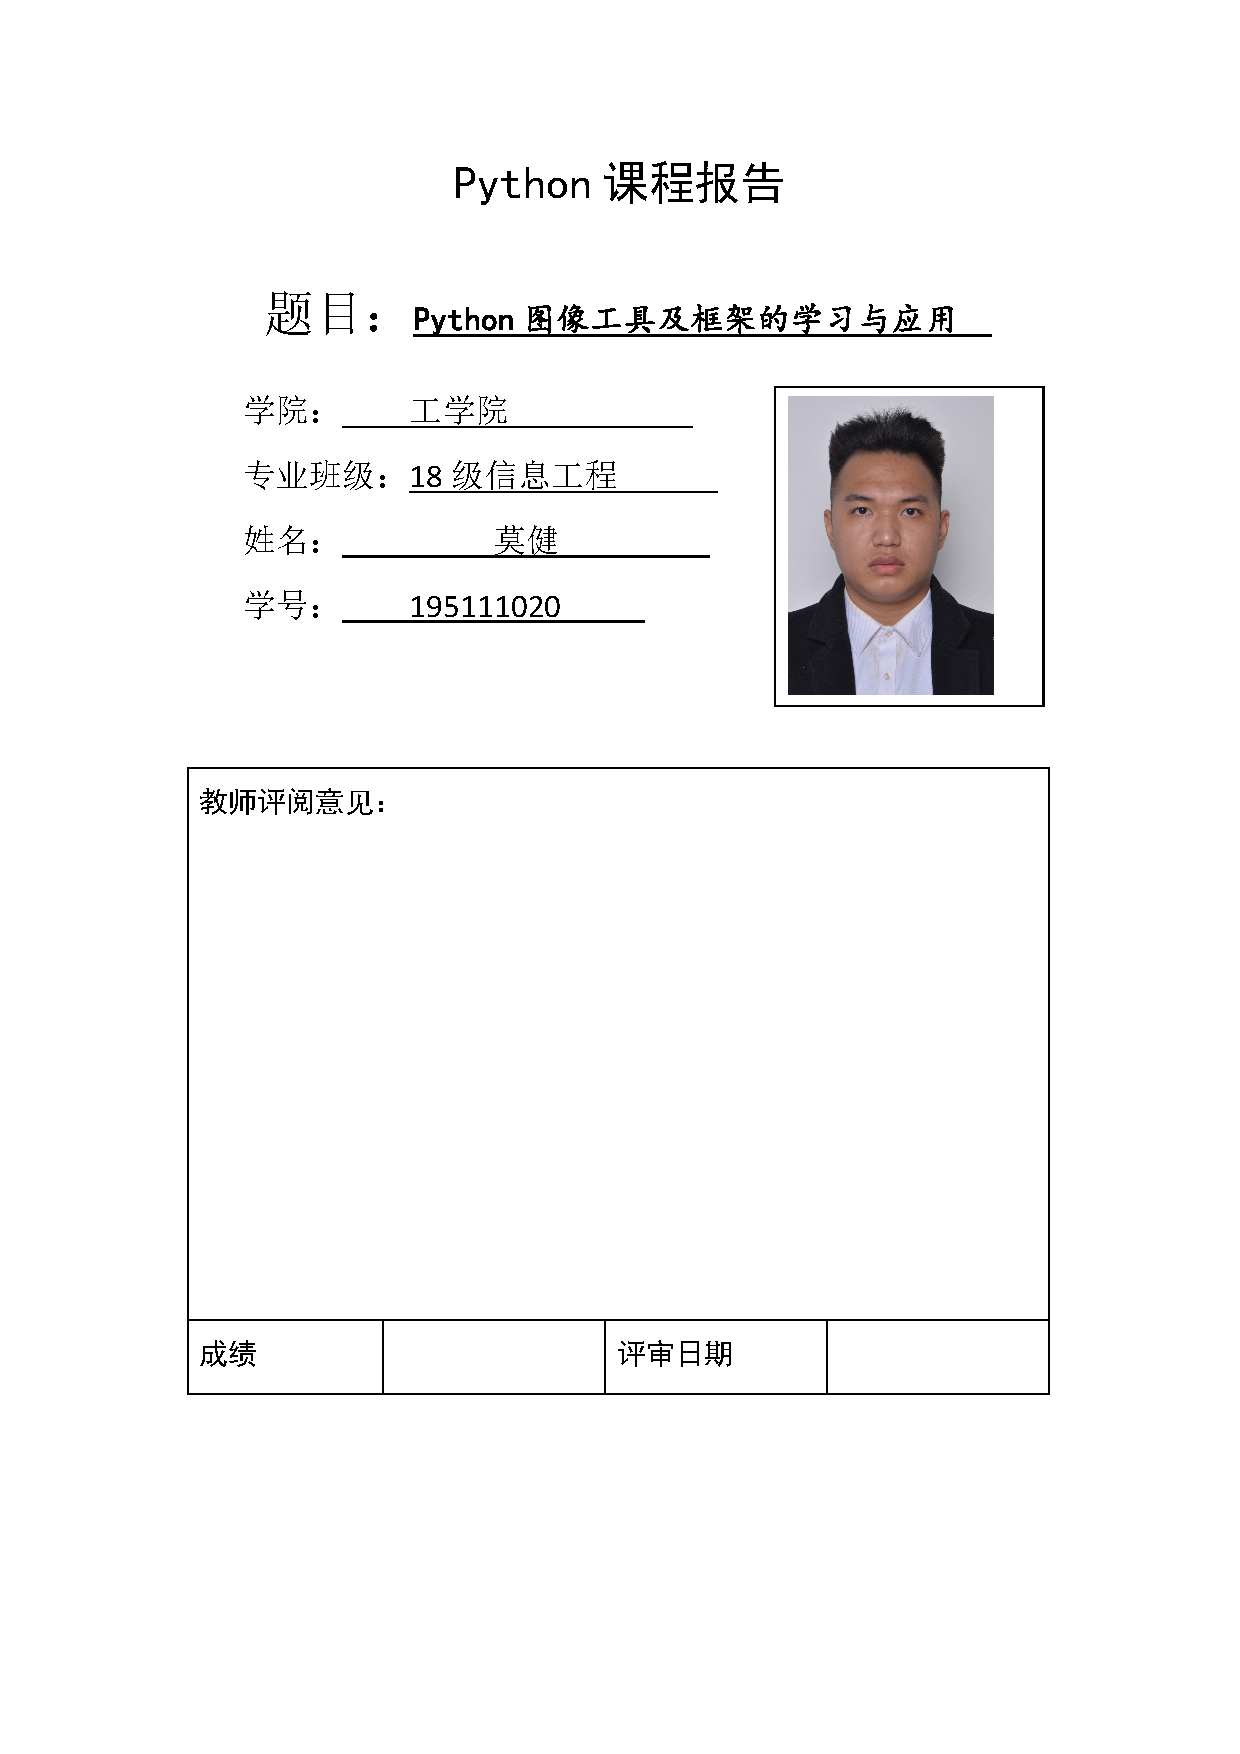
\includepdf[pages=-]{../figure/py/cover.pdf}
\begin{abstract}
本文列举了Python处理图像的实用工具或框架, 简述了前景背景分离的原理, 经典算法和常用框架, 并尝试使用这些框架尝试处理了图片. 
\end{abstract}
\section{常用的图像处理库}
Python中有许多常用的图像处理库\cite{web:tools}, 这其中有部分是从科学计算, 矩阵处理中通用库; 也有专注于图像处理的软件包. 
\subsection{科学计算库}
\subsubsection{NumPy}
NumPy是Python编程中的核心库之一,提供对数组的支持。图像本质上是一个标准的NumPy数组,包含数据点的像素。因此,通过使用基本的NumPy操作,如切片、蒙版和花式索引,可以修改图像的像素值。可以使用skimage加载图像,使用Matplotlib显示图像。
\subsubsection{SciPy}
SciPy是Python的另一个核心科学模块(和NumPy一样),可以用于基本的图像操作和处理任务。特别是子模块scipy.ndimage提供了在n维NumPy数组上操作的函数。该软件包目前包括线性和非线性滤波、二元形态、B-spline插值和对象测量的函数。
\subsubsection{Matplotlib}
Matplotlib主要用于二维可视化,但它也可以用于图像处理。虽然它不支持所有的文件格式,但Matplotlib可以有效地调整图像,从中提取信息。
\subsection{图像库}
\subsubsection{scikit-image}
scikit-image是一个开源的Python包。它实现了用于研究、教育和工业应用的算法和实用程序。它是一个相当简单和直接的库,即使对于那些刚接触Python生态系统的人来说也是如此。其代码是高质量的,经过同行评审的,由一个活跃的志愿者社区编写。

scikit-image通过转换原始图片,使用NumPy数组作\footnote{这些NumPy数组既可以是整数(有符号或无符号),也可以是浮点数。}为图像对象。而且由于NumPy是用C语言编程建立的,所以速度非常快,使其成为图像处理的十分理想的库。
\subsubsection{Mahotas}
Mahotas是一个Python的计算机视觉和图像处理和操作库。一个库是一个函数和方法的集合,它允许你执行许多操作,而不需要编写数百行代码。Mahotas包含了许多用数组操作的算法,目前Mahotas有100多个用于图像处理和计算机视觉的函数,并且还在不断增加。

Mahotas在寻找图像中的重复图案方面提供了很好的解决方案,例如 "Where's Wally Problem "就可以用Mahotas轻松解决。
\subsubsection{Pillow}
许多非科学的Python项目都利用PIL或Pillow。例如,Python网络框架Django使用PIL来表示数据库中的图像区域。如果你需要做一些快速但不优雅的图像处理,PIL和Pillow有它们的位置,但如果需要认真地学习图像处理、计算机视觉和图像搜索引擎,往往会其他有更好的选择.
\subsubsection{OpenCV}
OpenCV\footnote{Open Source Computer Vision Library}是计算机视觉应用最广泛的库之一。OpenCV支持多种编程语言,如C++、Python、Java等,并可在Windows、Linux、OS X、Android和iOS等不同平台上使用。基于CUDA和OpenCL的高速GPU操作接口也在积极开发中。

OpenCV-Python是OpenCV的Python API。OpenCV-Python不仅速度快,因为后台由C/C++编写的代码组成,而且它还易于编码和部署(由于前台的Python封装器)。这使得它成为执行计算密集型计算机视觉程序的绝佳选择。


\subsubsection{SimpleCV}
SimpleCV是另一个用于构建计算机视觉应用程序的开源框架,它提供了对OpenCV等多个功能强大的计算机视觉库的访问,但不必了解位深、文件格式、色彩空间等。它提供了对OpenCV等几个高功能计算机视觉库的访问,但不必了解位深、文件格式、色彩空间等。它的学习曲线大大小于OpenCV的学习曲线,正如其名称所言,它使得计算机视觉变得简单。
\subsubsection{h5py}
h5py库是Python中存储大型数值数据集的库。它提供了对 NumPy 数组的支持。如果你有一个大型的数据集用 NumPy 数组表示,而且它不适合放在内存中,或者你想要高效、持久地存储 NumPy 数组,那么 h5py 是你的最佳选择。整个数据集永远不需要一次性从磁盘上完全加载,而且内存占用非常小,即使是数千个特征向量也是如此。
\section{前景背景分离技术}
影像去背(Image Matting)是一种很常见的图像处理应用\cite{matting}。简单来说,Matting就是保留图片中需要的像素,删除其他部分。所以可以将图片分为前景和背景两部分。借由计算前景的颜色和透明度,将前景从影像中撷取出来的技术,就被称为Image Matting, 可用于替换背景、影像合成、视觉特效,在电影工业中被广泛地使用。影像中的每个像素会有代表其前景透明度的值,称作阿尔法值(Alpha),一张影像中所有阿尔法值的集合称作阿尔法遮罩(Alpha Matte),将影像被遮罩所涵盖的部分取出即可完成前景的分离。
许多图像编辑和电影后期制作应用都依赖于自然图像去背作为处理步骤之一。matting算法的任务是准确估计图像或视频序列中前景物体的不透明度。


影像去背的主要工作就是求得精确的阿尔法遮罩(alpha matte),而影像常有无法人工标示的部分,例如:人的发丝或是动态模糊的部分,一种简单的解决方法是先人工标定出影像的“Trimap”,再由算法计算出阿尔法遮罩以完成影像去背。


概括出来就一个公式
\begin{align*}
  \underset{\text{图像}}{I} =\alpha\cdot \underset{\text{前景}}{F} +(1-\alpha)\cdot \underset{\text{背景}}{B} 
\end{align*}
\begin{figure}[H]
\centering
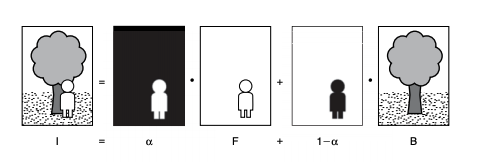
\includegraphics[width=1\textwidth]{matting_equ.png}
\caption{$I=\alpha\cdot F+(1-\alpha)\cdot B$ 的形象解释}
\end{figure}
当然,因为$F, B$和$\alpha$都是未知的,要把这么多未知项都求出来显然很不容易。所以就需要增加一些附加的约束,通常,这种约束以Trimap的形式给出。

融合系数$\alpha$是一个介于0到1之间的分数,它给出了前景和背景在待处理影象中所占的比例。显然,对于确定的背景部分,$\alpha=0$;对于确定的前景部分,$\alpha=1$。在前景与背景相互融合的边缘部分,$\alpha$基于0到1之间。而这正是最终要求解的核心问题。

\subsection{术语}
% \subsubsection{matting} 前背景分离
\subsubsection{color space} 色彩空间, 主要有RGB, CMYK和HSV. 当然也有灰度图. 一个在二维空间的点(图片)在RGB色彩空间下可以表示为
\begin{align*}
  I(x,y)=\begin{bmatrix}
    R\\
    G\\
    B
  \end{bmatrix}
\end{align*}这样一个向量
\paragraph{RGB} 
三原色光模式(RGB color model),又称RGB颜色模型或红绿蓝颜色模型,是一种加色模型,将红(Red)、绿(Green)、蓝(Blue)三原色的色光以不同的比例相加,以合成产生各种色彩光。若加上透明度通道可形成RGBA
\begin{figure}[H]
\centering
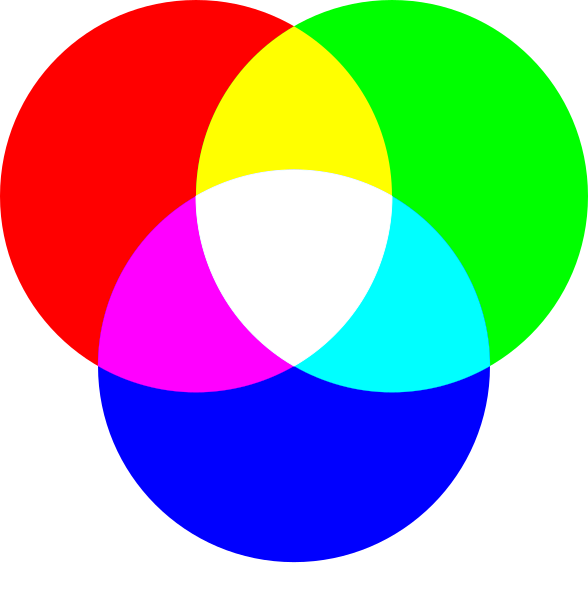
\includegraphics[width=0.33\textwidth]{rgb.png}
\caption{RGB}
\end{figure}
\paragraph{CMYK}
印刷四分色模式(CMYK)是彩色印刷时采用的一种套色模式,利用色料的三原色混色原理,加上黑色油墨,共计四种颜色混合叠加,形成所谓“全彩印刷”。
\begin{figure}[H]
\centering
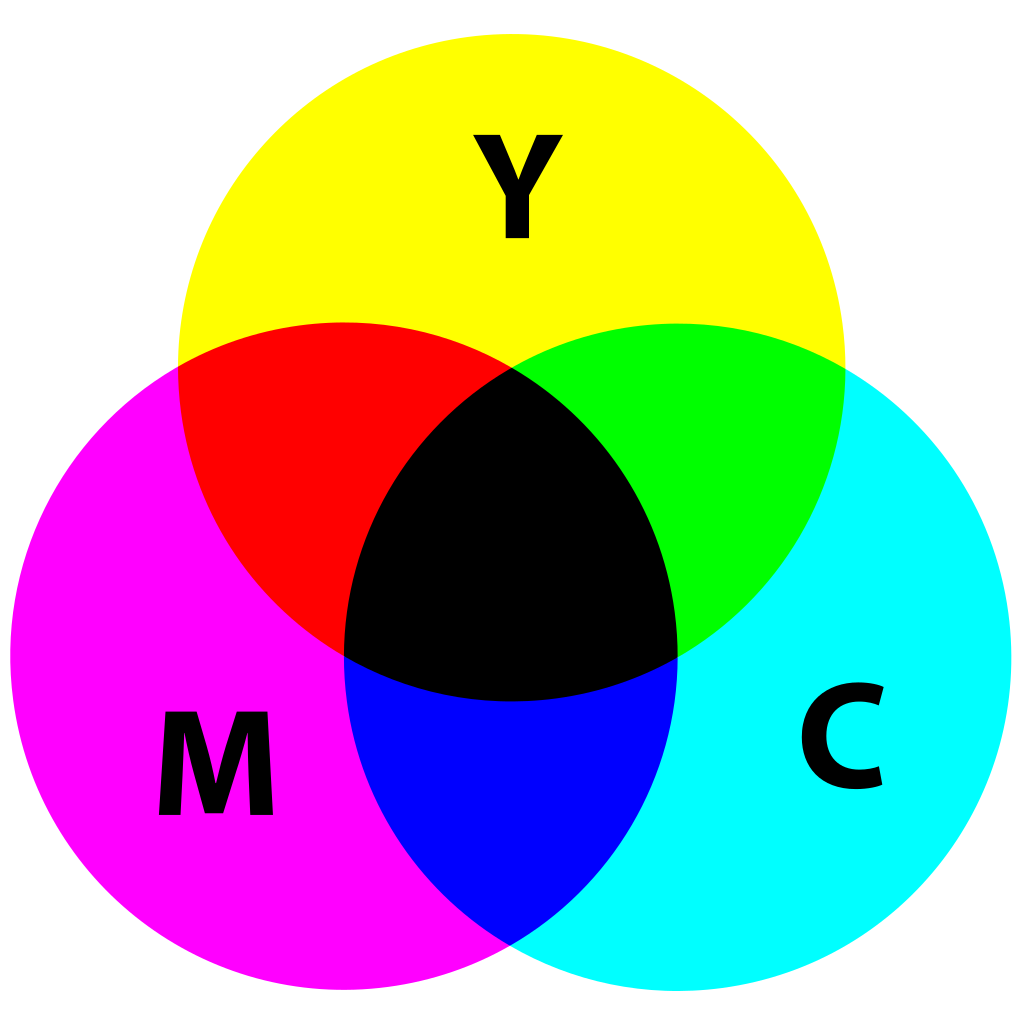
\includegraphics[width=0.33\textwidth]{cmyk.png}
\caption{CMYK}
\end{figure}
\begin{itemize}
  \item \textbf{C}yan 青色,常被误称为“天蓝色”或“湛蓝”
  \item \textbf{M}agenta 洋红色,又称为“品红色”
  \item \textbf{Y}ellow 黄色
  \item blac\textbf{K} 黑色,此处缩写使用最后一个字母K而非开头的B,是因为在整体色彩学中已经将B给了RGB的Blue蓝色。
\end{itemize}

\paragraph{HSV和HSL}
HSL和HSV都是一种将RGB色彩模型中的点在圆柱坐标系中的表示法。这两种表示法试图做到比基于笛卡尔坐标系的几何结构RGB更加直观。

\begin{figure}[H]
\centering
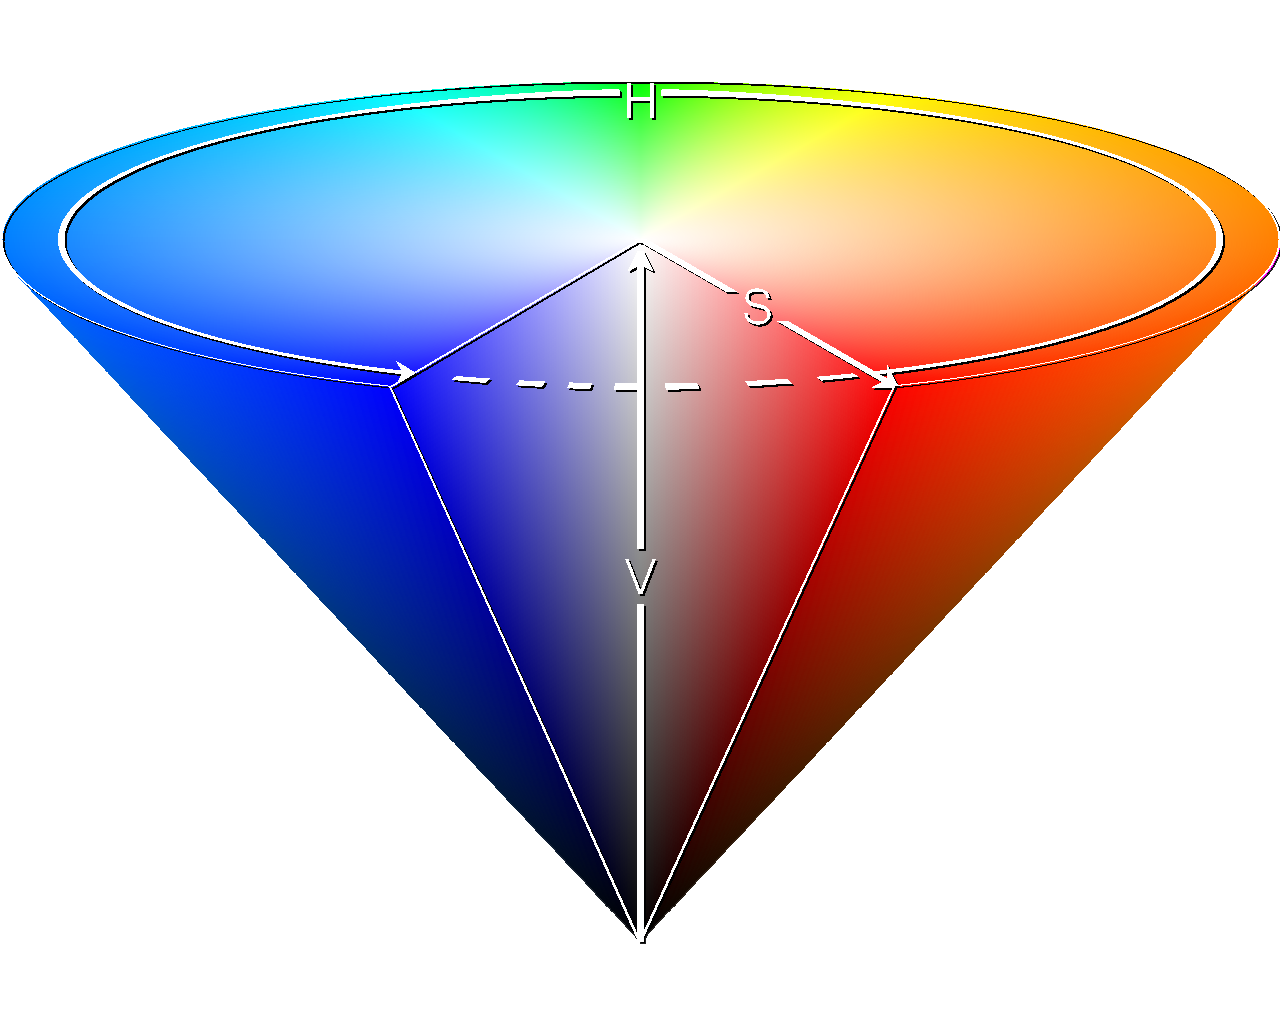
\includegraphics[width=0.33\textwidth]{HSV_cone.png}
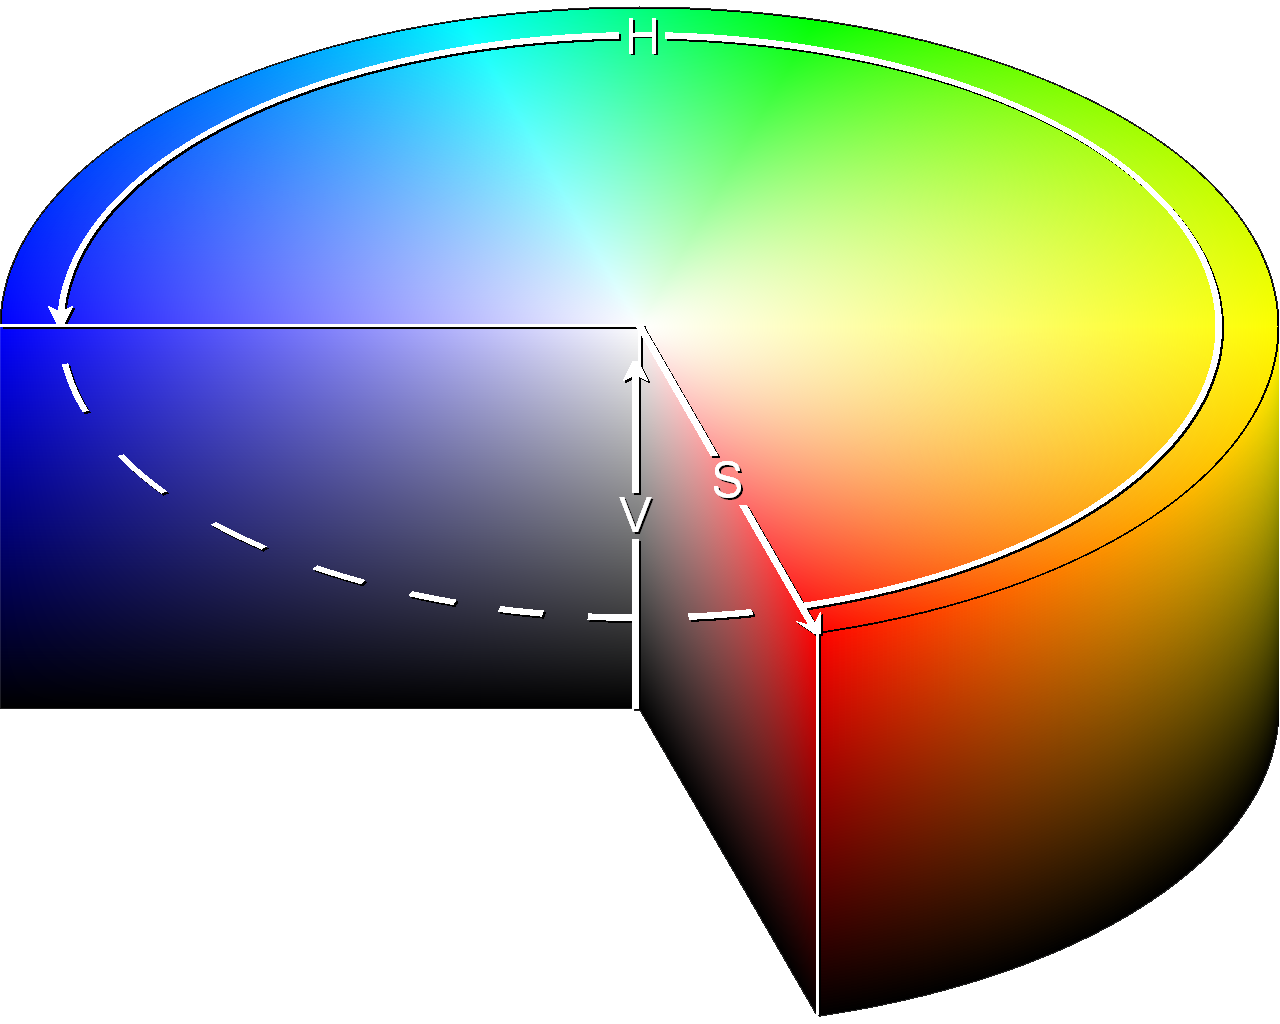
\includegraphics[width=0.33\textwidth]{HSV_cylinder.png}
\caption{HSV(左图)和HSL(右图)}
\end{figure}
HSL即色相、饱和度、亮度(英语:Hue, Saturation, Lightness)。HSV即色相、饱和度、明度(英语:Hue, Saturation, Value),又称HSB,其中B即英语:Brightness。
\begin{itemize}
  \item 色相(H)是色彩的基本属性,就是平常所说的颜色名称,如红色、黄色等。
  \item 饱和度(S)是指色彩的纯度,越高色彩越纯,低则逐渐变灰,取0-100\%的数值。  
  \item 明度(V),亮度(L),取0-100\%。 
\end{itemize}
\subsubsection{alpha matte} 透明度遮罩\cite{matting} (阿尔法遮罩),是代表对于影像前景透明度的遮罩,大小和影像相同,遮罩中每个像素的值为相应的影像像素的阿尔法值(Alpha)。阿尔法值为1代表该像素属于前景,0则代表该像素属于背景。阿尔法值也可能介于0,1之间,表示对应到的影像像素为半透明,例如烟雾、动态模糊。
\begin{figure}[H]
\centering
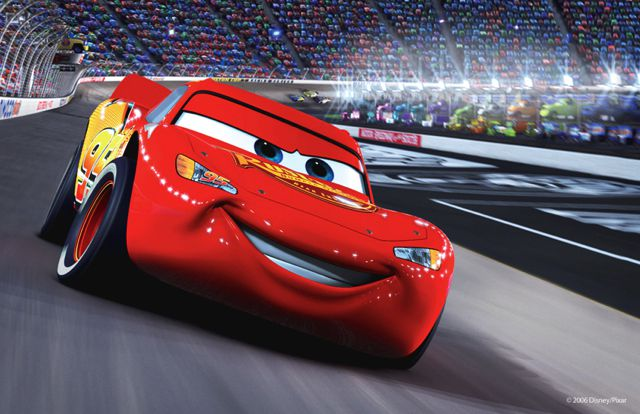
\includegraphics[width=0.33\textwidth]{source13_compressed.jpg}
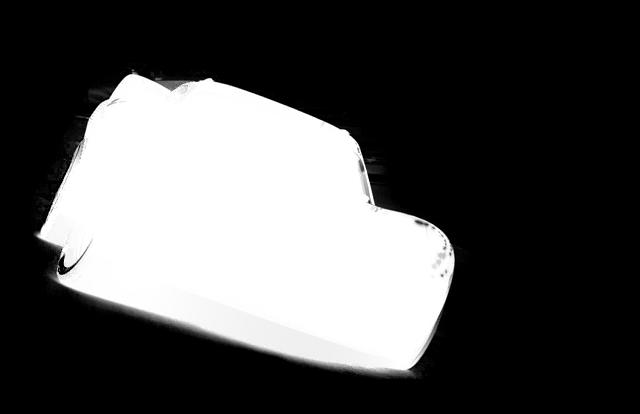
\includegraphics[width=0.33\textwidth]{alpha013.jpg}
\caption{Alpha matte (右图)}
\end{figure}
\subsubsection{trimap} 又被译作三分图, 三值模板\cite{matting}. 一张影像的“Trimap”,是指将影像中的每个像素划分为三种区域:前景(Foreground)、背景(Background)和待确认(Unknown)。算法会将标定好的前景和背景当成已知,再借由颜色等资讯将待确认区域中的像素标为前景或背景。
\begin{figure}[H]
\centering
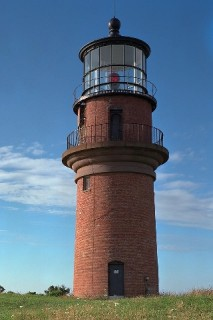
\includegraphics[width=.2\textwidth]{tower.jpg}
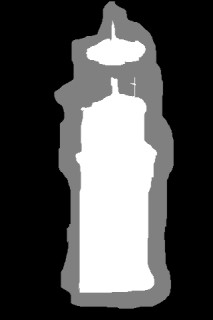
\includegraphics[width=.2\textwidth]{trimap.jpg}
\caption{Trimap (右图)}
\end{figure}
右图中黑色为背景, 白色为前景, 而灰色就是待确认部分. 
\subsubsection{scribble} 简单标记\cite{matting}, 随便在原图划拉两下.黑色表示背景,白色表示前景. 
\begin{figure}[H]
\centering
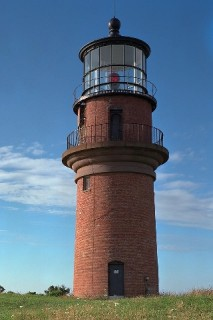
\includegraphics[width=0.2\textwidth]{tower.jpg}
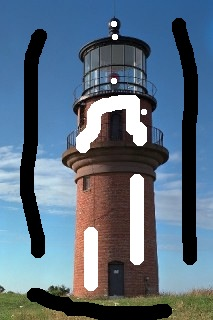
\includegraphics[width=0.2\textwidth]{scribble.jpg}
\caption{scribble (右图)}
\end{figure}

\subsection{算法}
% 可大致分为两类:取样法(Sampling-based)和传播法(Propagation-based)。
\subsubsection{取样法}
取样法 (Sample-based image matting) 会对影像的局部区域取样,从已知资讯计算出该区域的阿尔法遮罩。常见的方法有Bayesian Matting。

\paragraph{Bayesian Matting}
以贝叶斯计算最大后验概率,对前景、背景及阿尔法值同步进行优化,使用有向高斯共变异数(Oriented Gaussian Covariances)能有效的推估颜色的分布。贝氏去背的优点是几率模型简单又符合直觉,去背效果良好。其限制是需要良好的“Trimap”,当影像的前后景关系变得复杂时,贝叶斯去背的效果会显著下降

在融合方程中,已知的只有$C$,而$F, B$和α$\alpha$都是未知的。于是可以从条件概率的角度去考虑这个问题,即给定$C$时,$F, B$和α$\alpha$的联合概率应为
\begin{align*}
  P(F,B,\alpha\mid C)
  &=\frac{P(C\mid F,B,\alpha)\cdot P(F,B,\alpha)}{P(C)}\\
  &=\frac{P(C\mid F,B,\alpha)\cdot P(F)\cdot P(B)\cdot P(\alpha)}{P(C)}
\end{align*}
其中第一个等号是根据贝叶斯公式得到的,第二个等号则是考虑$F, B$和$\alpha$是彼此独立的。上式表明Matting问题可以被转化为已知待计算画素颜色C的情况下,如何估计它的$F, B$和$\alpha$的值以最大化后验概率$P(F,B,\alpha\mid C)$的问题。

上述等式中的右端项,需要通过取样统计的方式进行估计,而这种估计结果的准确性,很大程度上决定了算法的融合质量。具体来说,算法采用一个连续滑动的视窗对邻域进行取样,视窗从未知区域和己知区域之间的两条边开始向内逐轮廓推进,计算过程也随之推进。
\subsubsection{传播法}
传播法(Propagation image matting)是指借由分析整张影像的特性,像是颜色、梯度等,来直接求得整张影像遮罩的方法。常见的方法有Poisson Matting、Robust Matting等。
\paragraph{Poisson Matting}
帕松去背分为两步,一是从影像中算出遮罩近似的梯度场,二是借由解帕松等式(Poisson Equation),从遮罩的梯度场求得遮罩。当前景和背景颜色接近时,帕松去背容易出错,此时能够以更多的使用者输入,用区域的帕松去背来进行优化。
\paragraph{Robust Matting}
通常在有品质好的“Trimap”的情况下,取样法可以得到较好的遮罩;但在前后景关系复杂,“Trimap”品质不佳时,取样法的效果会迅速衰减。稳健性去背景法会先进行取样,得到遮罩后再进行优化,进而结合取样法和传播法的好处。
\subsubsection{机器学习}
大多数现有的去背方法需要绿幕背景或手动创建的"Trimap"来产生良好的去背。自动的、无"Trimap"的方法正在出现,但其质量仍然不够好。某些基于机器学习的matting算法,要求用户在拍摄时额外拍摄一张没有主体的背景照片。这一步需要少量的操作,但远比创建"Trimap"耗时少。
\begin{itemize}
  \item \href{https://ieeexplore.ieee.org/document/6409354}{KNN Matting - IEEE}
  \item \href{https://arxiv.org/abs/1703.03872}{Deep Image Matting}
  \item \href{https://github.com/senguptaumd/Background-Matting}{Background Matting: The World is Your Green Screen}
  \item \href{http://alphamatting.com/}{alphamatting.com}
\end{itemize}
% \paragraph{KNN Matting}
% \href{https://ieeexplore.ieee.org/document/6409354}{KNN Matting - IEEE}
% \paragraph{Deep Image Matting}
% \href{https://arxiv.org/abs/1703.03872}{Deep Image Matting}
% \paragraph{Background Matting}
% \href{https://github.com/senguptaumd/Background-Matting}{Background Matting: The World is Your Green Screen}
% \paragraph{训练数据集} \href{http://alphamatting.com/}{alphamatting.com}
\subsection{辅助方法}
在实际操作中,可以借由增加观测资讯,让去背景变得更加容易。
\subsubsection{红外线}
在拍摄时,同时使用一般镜头和红外线镜头,借由红外线照片所得到的资讯,将同时拍摄的一般照片当中的人与背景分离。
\subsubsection{闪光}
在拍摄时,拍下使用闪光灯和没有使用闪光灯各一张,闪光灯会明显改变前景的亮度,但对背景的影响较小,借由分析有无闪光的两张照片,来完成影像去背。
\subsection{影像前景背景分离技术}
如果可以给定多张图像 (视频), 我们就可以利用运动分析(Motion analysis) 和 物体追踪(Object tracking)来进行前景背景分离. 

前景检测 (Foreground detection)是计算机视觉和图像处理领域的主要任务之一,其目的是检测图像序列的变化。背景去除(Background subtraction)就是任何允许提取图像的前景以进行进一步处理(物体识别等)的技术。

许多应用不需要知道视频序列中运动演变的所有信息,而只需要知道场景的变化信息,因为图像的兴趣区是其前景的物体(人、车、文字等)。在图像预处理阶段(可能包括图像去噪、形态学\footnote{\href{https://en.wikipedia.org/wiki/Mathematical_morpholog}{Mathematical morphology}}等后期处理)后,需要进行物体定位,这可能会利用这种技术。

前景检测根据前景发生的这些变化将前景和背景分开。它是一套典型的分析用固定摄像机实时记录的视频序列的技术。
\subsubsection{算法}
OpenCV中自带有\href{https://docs.opencv.org/master/de/de1/group__video__motion.html}{几个算法}和\href{https://docs.opencv.org/master/d1/dc5/tutorial_background_subtraction.html}{示例代码}
\begin{itemize}
  \item MOG
  \item MOG2
  \item GMG 
  \item KNN
  \item CNT
\end{itemize}
\section{前景背景分离实践}

% \begin{figure}[H]
% \centering
% \includegraphics[width=0.23\textwidth]{img/test_resize.jpg}
% \includegraphics[width=0.23\textwidth]{img/test_removebg.png}
% \includegraphics[width=0.23\textwidth]{img/removebg_cutout.png}
% \includegraphics[width=0.23\textwidth]{img/removebg_orig_bg.png}
% \caption{从左至右分别是原图, Alpha遮罩, 得到的前景和背景}
% \label{fig:ideal}
% \end{figure}

本次实践使用了\href{https://www.remove.bg/}{removebg}的API生成的图片作为测试基准, 如图~\ref{fig:ideal}所展示的效果. 

\begin{figure}[H]
  \centering
  \begin{subfigure}{0.23\textwidth}
    \centering
    \includegraphics[width=\textwidth]{img/test_resize.jpg}
    \caption{原图}
  \end{subfigure}
  \begin{subfigure}{0.23\textwidth}
    \centering
    \includegraphics[width=\textwidth]{img/removebg_cutout.png}
    \caption{Cutout}
  \end{subfigure}
  \begin{subfigure}{0.23\textwidth}
    \centering
    \includegraphics[width=\textwidth]{img/test_removebg.png}
    \caption{Alpha遮罩}
    \label{fig:alpha_eg}
  \end{subfigure}
  \begin{subfigure}{0.23\textwidth}
    \centering
    \includegraphics[width=\textwidth]{img/removebg_orig_bg.png}
    \caption{背景图}
  \end{subfigure}

  \caption{使用removebg API的处理示例}
  \label{fig:ideal}
  \end{figure}


因得到的背景图像的实用价值较前景来说较低, 故以下省略了分离之后的背景的展示(如图~\ref{fig:ideal}最右图), 而增加一项使用新的背景图来替代原图的测试 (如图~\ref{fig:blended}). 
% \begin{figure}[H]
% \centering
% \includegraphics[width=0.3\textwidth]{img/test_resize.jpg}
% \includegraphics[width=0.3\textwidth]{img/bg_rz.png}
% \includegraphics[width=0.3\textwidth]{img/removebg_blended.png}
% \caption{从左至右分别为原图, 新增背景图和混合之后的图像}
% \label{fig:blended}
% \end{figure}

\begin{figure}[H]
  \centering
  \begin{subfigure}{0.32\textwidth}
    \centering
    \includegraphics[width=\textwidth]{img/test_resize.jpg}
    \caption{原图}
  \end{subfigure}
  \begin{subfigure}{0.32\textwidth}
    \centering
    \includegraphics[width=\textwidth]{img/bg_rz.png}
    \caption{背景图}
  \end{subfigure}
  \begin{subfigure}{0.32\textwidth}
    \centering
    \includegraphics[width=\textwidth]{img/removebg_blended.png}
    \caption{合成图像}
  \end{subfigure}

  \caption{背景图处理示例}
  \label{fig:blended}
  \end{figure}

\subsection{GrabCut}
GrabCut算法\cite{rother2004grabcut}利用了图像中的纹理(颜色)信息和边界(反差)信息,只要少量的用户交互操作即可得到比较好的分割结果。只需要在目标外面画一个框,把目标框住,它就可以完成良好的分割; 因为GrabCut是按颜色分布和边缘对比度来分割图片的,对一些常见的与此原则相悖的图片,效果确实不好。比如前景人物的帽子、鞋、墨镜,通常颜色跟前景主体有较大区别;再如前景中的孔,有可能由于颜色区分和边缘的对比度不足,导致边缘的惩罚占上风,而没有扣出来背景。
\begin{figure}[H]
\centering
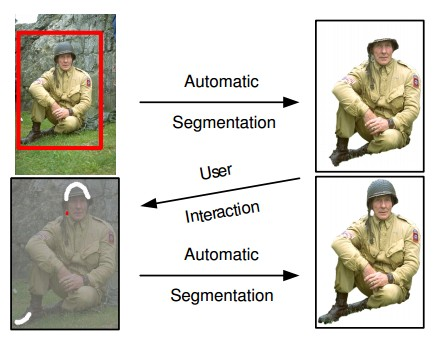
\includegraphics[width=0.6\textwidth]{grabcut.jpg}
\caption{GrabCut的User Edit方法}
\label{fig:grabcut_edit}
\end{figure}
所以,GrabCut还是保留了人工修正的操作,定义了两种标记:绝对是背景和可能是前景。对分割错误人工修正后(如图~\ref{fig:grabcut_edit})\footnote{时间所限, 本次实践对user edited修正方法尚未涉及},分割还是可以比较准确的。 

参考官方文档 \href{https://docs.opencv.org/master/dd/dfc/tutorial_js_grabcut.html}{Foreground Extraction using GrabCut Algorithm}
, 代码见\lstinline{grabcut.py}

\begin{figure}[H]
  \centering
  \begin{subfigure}{0.23\textwidth}
    \centering
    \includegraphics[width=\textwidth]{img/test_resize.jpg}
    \caption{原图}
  \end{subfigure}
  \begin{subfigure}{0.23\textwidth}
    \centering
    \includegraphics[width=\textwidth]{img/output/grabcut_withline.jpg}
    \caption{带范围框的原图}
  \end{subfigure}
  \begin{subfigure}{0.23\textwidth}
    \centering
    \includegraphics[width=\textwidth]{img/output/grabcut_alpha.jpg}
    \caption{Alpha遮罩}
  \end{subfigure}
  \begin{subfigure}{0.23\textwidth}
    \centering
    \includegraphics[width=\textwidth]{img/output/grabcut_blended.jpg}
    \caption{合成图像}
  \end{subfigure}

  \caption{GrabCut算法的处理结果}
  \end{figure}

% \begin{figure}[H]
% \centering
% \includegraphics[width=.23\textwidth]{img/test_resize.jpg}
% \includegraphics[width=.23\textwidth]{img/output/grabcut_withline.jpg}
% \includegraphics[width=.23\textwidth]{img/output/grabcut_alpha.jpg}
% \includegraphics[width=.23\textwidth]{img/output/grabcut_blended.jpg}
% \caption{GrabCut得到的处理结果. 从左到右依次为原图, 带范围框的原图, Alpha透明度遮罩和混合图像}
% \end{figure}


\subsection{PyMatting}
Github文档见\href{https://github.com/pymatting/pymatting}{A Python Library for Alpha Matting}\cite{germer2020pymatting}. 

给定一个输入图像和一个手绘或者自动生成的Trimap,使用Alpha去背方法估计前景对象的Alpha通道 (Alpha透明度遮罩),然后可以组成不同的背景。

PyMatting提供以下Alpha去背方法
\begin{itemize}
  \item Closed Form Alpha Matting
  \item Large Kernel Matting 
  \item KNN Matting
  \item Learning Based Digital Matting
  \item Random Walk Matting
\end{itemize}
和以下前景估计实现
\begin{itemize}
  \item Closed Form Foreground Estimation 
  \item Fast Multi-Level Foreground Estimation 
\end{itemize}

本示例中使用了Closed Form Alpha Matting\cite{4359322} 方法\footnote{\lstinline{alpha.estimate_alpha_cf}函数} (由于时间所限, 尚未测试其他方法), 代码见\lstinline{pymat.py}
% \begin{figure}[H]
% \centering
% 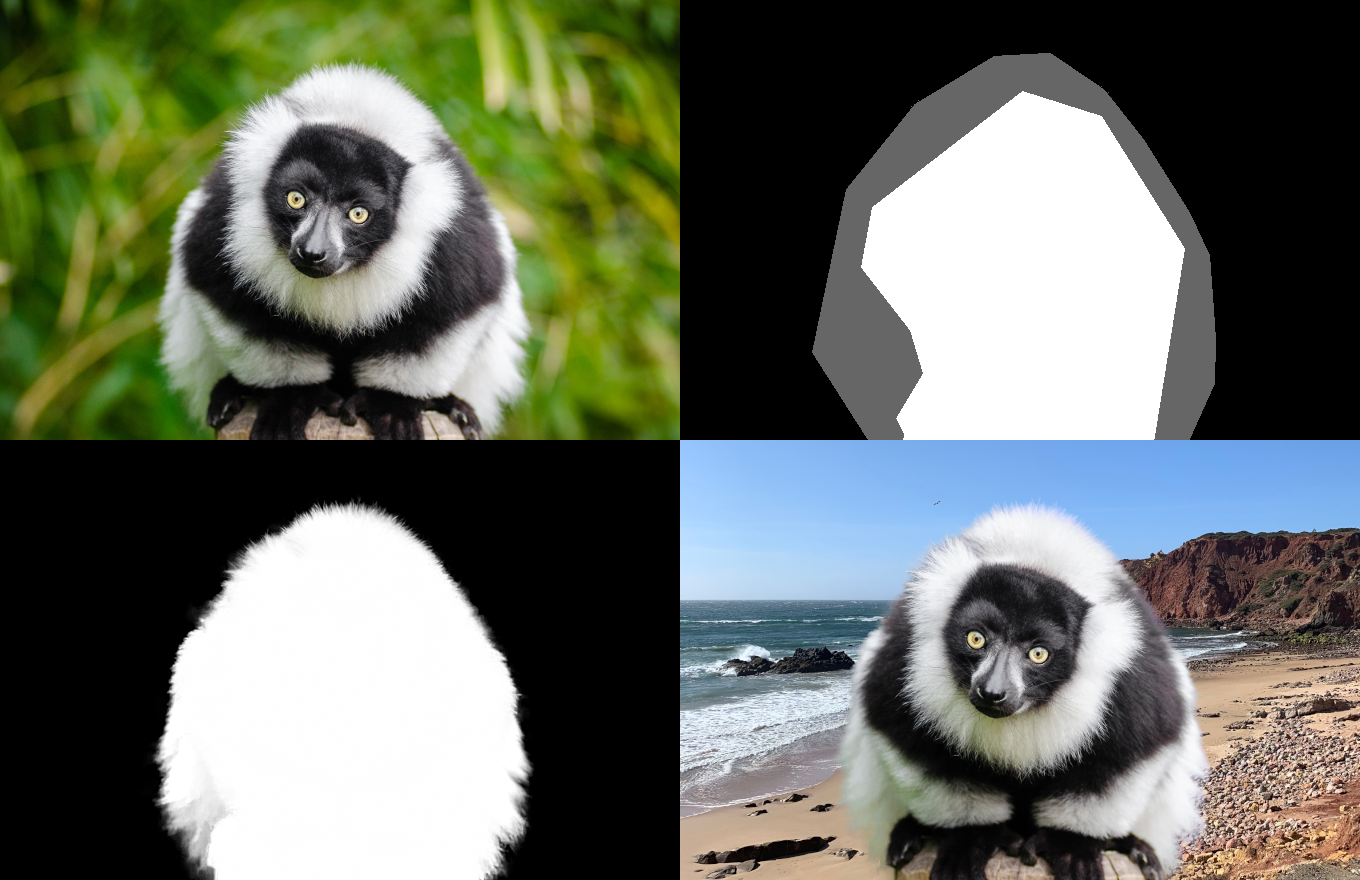
\includegraphics[width=.8\textwidth]{lemur_at_the_beach.png}
% \caption{「沙滩上的狐猴」PyMatting官方示例图像}
% \end{figure}
% \begin{figure}[H]
% \centering
% \includegraphics[width=.23\textwidth]{img/test_resize.jpg}
% \includegraphics[width=.23\textwidth]{img/test_trimap.png}
% \includegraphics[width=.23\textwidth]{img/output/trimap_alpha.png}
% \includegraphics[width=.23\textwidth]{img/output/trimap_blended.png}
% \caption{PyMatting中的Closed Form Alpha Matting方法得到的处理结果. 从左到右依次为原图, Trimap, Alpha透明度遮罩和混合图像}
% \end{figure}

\begin{figure}[H]
  \centering
  \begin{subfigure}{0.23\textwidth}
    \centering
    \includegraphics[width=\textwidth]{img/test_resize.jpg}
    \caption{原图}
  \end{subfigure}
  \begin{subfigure}{0.23\textwidth}
    \centering
    \includegraphics[width=\textwidth]{img/test_trimap.png}
    \caption{Trimap}
  \end{subfigure}
  \begin{subfigure}{0.23\textwidth}
    \centering
    \includegraphics[width=\textwidth]{img/output/trimap_alpha.png}
    \caption{Alpha遮罩}
  \end{subfigure}
  \begin{subfigure}{0.23\textwidth}
    \centering
    \includegraphics[width=\textwidth]{img/output/trimap_blended.png}
    \caption{合成图像}
  \end{subfigure}

  \caption{PyMatting库的处理结果}
  \end{figure}


\subsubsection{Trimap的处理}
通常我们得到的Trimap可能会包含不止三种\footnote{黑, 白和50\%灰之外可能会因为图像处理软件的抗锯齿算法混进去其他颜色}种颜色. 直接丢进去PyMatting会报错, 故需要进行预处理得到只有三种颜色的Trimap. 
PyMatting已经自带有\href{https://pymatting.github.io/pymatting.util.html?highlight=trimap\#pymatting.util.util.fix\_trimap}{\lstinline{ fix\_trimap}}函数. 就是根据
\begin{align*}
  T_{\text{fixed}}=\begin{cases}
    0, &T<\text{上阈值}\\
    \frac{1}{2},&\text{其他}\\
    1. &T>\text{下阈值}
  \end{cases}
\end{align*}
计算得到的
\subsubsection{背景提取}
值得注意的是PyMatting中的\href{https://pymatting.github.io/pymatting.foreground.html?highlight=estimate\#module-pymatting.foreground.estimate\_foreground\_ml}{\lstinline{foreground.estimate\_foreground\_ml module}}函数\footnote{即上文提到的Fast Multi-Level Foreground Estimation的实现}可以返回经过估计的背景 (而非留黑), 如图~\ref{fig:pym_bg}所示.  
\begin{figure}[H]
\centering
\includegraphics[width=0.33\textwidth]{img/test_resize.jpg}
\includegraphics[width=0.33\textwidth]{img/output/trimap_bg_orig.png}
\caption{左图为原图, 右图为估计背景}
\label{fig:pym_bg}
\end{figure}
% \subsubsection{Color Bleeding}
% 在计算机图形和三维渲染中, Color Bleeding是指物体或表面被附近表面的有色光反射而着色的现象。

\subsection{Close-Form Matting}

Github文档见\href{https://github.com/MarcoForte/closed-form-matting}{Closed-Form Matting}

就是上文PyMatting库的Closed Form Alpha Matting\cite{4359322}另一个库的实现, 可以做到根据scribble
%\footnote{简单标记, 随便在原图划拉两下. 黑色表示背景, 白色表示前景}
就能进行前景背景分离, 虽然最后的效果不如前两者理想. 


代码见\lstinline{closed_form.py}

\begin{figure}[H]
  \centering
  \begin{subfigure}{0.23\textwidth}
    \centering
    \includegraphics[width=\textwidth]{img/test_resize.jpg}
    \caption{原图}
  \end{subfigure}
  \begin{subfigure}{0.23\textwidth}
    \centering
    \includegraphics[width=\textwidth]{img/test_scribble.png}
    \caption{Scribble}
  \end{subfigure}
  \begin{subfigure}{0.23\textwidth}
    \centering
    \includegraphics[width=\textwidth]{img/output/scribble_alpha.png}
    \caption{Alpha遮罩}
  \end{subfigure}
  \begin{subfigure}{0.23\textwidth}
    \centering
    \includegraphics[width=\textwidth]{img/output/scribble_blended.png}
    \caption{合成图像}
  \end{subfigure}

  \caption{Close-Form Matting库的处理结果}
  \end{figure}

% \begin{figure}[H]
% \centering
% \includegraphics[width=.23\textwidth]{img/test_resize.jpg}
% \includegraphics[width=.23\textwidth]{img/test_scribble.png}
% \includegraphics[width=.23\textwidth]{img/output/scribble_alpha.png}
% \includegraphics[width=.23\textwidth]{img/output/scribble_blended.png}
% \caption{Close-Form Matting库得到的处理结果. 从左到右依次为原图, 带Scribble的原图, Alpha透明度遮罩和混合图像}
% \end{figure}

\subsection{性能比较}
本次主要从处理时间和结构相似性指标两个方面对以上介绍的三种方法进行性能上的比较. 当然还有其他指标没有涉及到, 如处理时的内存占用以及MSE, PSNR等参数. 
\subsubsection{处理时间}
使用Powershell自带命令\href{https://docs.microsoft.com/en-us/powershell/module/microsoft.powershell.utility/measure-command?view=powershell-7}{\lstinline{ Measure-Command}}进行计时. 结果如图~\ref{fig:time}. 
\begin{figure}[H]
\centering
\begin{tikzpicture}
  \begin{axis}[
    xbar,
    % y axis line style = { opacity = 0 },
    % axis x line       = none,
    axis y line* =left,
    axis x line =bottom,
    tickwidth         = 0pt,
    enlarge y limits  = 0.2,
    enlarge x limits  = 0.02,
    symbolic y coords = {GrabCut, PyMatting, Close-Form Matting},
    ytick=data,
    nodes near coords,
    xlabel={time/second},
  ]
  \addplot coordinates { (6.4298356,GrabCut) (6.570087,PyMatting) (40.201513,Close-Form Matting)};
  \end{axis}
\end{tikzpicture}
\caption{处理所需时间 (越短越好)}
\label{fig:time}
\end{figure}
\subsubsection{SSIM}
结构相似性指标(structural similarity index,SSIM index)\cite{2004ITIP...13..600W}是一种用以衡量两张数位影像相似程度的指标。当两张影像其中一张为无失真影像,另一张为失真后的影像,二者的结构相似性可以看成是失真影像的影像品质衡量指标。
$$\text{SSIM}(x,y)={\frac {(2\mu _{x}\mu _{y}+c_{1})(2\sigma _{xy}+c_{2})}{(\mu _{x}^{2}+\mu _{y}^{2}+c_{1})(\sigma _{x}^{2}+\sigma _{y}^{2}+c_{2})}}$$
\begin{itemize}
  \item $\mu$ 表示均值
  \item $\sigma$ 表示方差 (协方差)
\end{itemize}
scikit-image已经包含了\href{https://scikit-image.org/docs/stable/api/skimage.measure.html?highlight=compare\_ssim\#skimage.measure.compare\_ssim}{\lstinline{compare\_ssim}} 
函数. 将基准图像的Alpha遮罩(图~\ref{fig:alpha_eg})和其余算法的结果进行对比, 结果如图~\ref{fig:ssim}. 

代码见\lstinline{compare.py}

\begin{figure}[hbt]
  \centering
  \begin{subfigure}{0.23\textwidth}
    \centering
    \includegraphics[width=\linewidth]{img/test_removebg.png}
    \caption{基准图像}
  \end{subfigure}
  \begin{subfigure}{0.23\textwidth}
    \centering
    \includegraphics[width=\linewidth]{img/output/grabcut_alpha.jpg}
    \caption{GrabCut}
  \end{subfigure}
  \begin{subfigure}{0.23\textwidth}
    \centering
    \includegraphics[width=\linewidth]{img/output/trimap_alpha.png}
    \caption{PyMatting}
  \end{subfigure}
  \begin{subfigure}{0.23\textwidth}
    \centering
    \includegraphics[width=\linewidth]{img/output/scribble_alpha.png}
    \caption{Close-Form Matting}
  \end{subfigure}
  % \includegraphics[width=.23\textwidth]{img/output/grabcut_alpha.jpg}
  % \includegraphics[width=.23\textwidth]{img/output/trimap_alpha.png}
  % \includegraphics[width=.23\textwidth]{img/output/scribble_alpha.png}
  % \includegraphics[width=0.32\textwidth]{img/diff/grabcut_diff.png}
  % \includegraphics[width=0.32\textwidth]{img/diff/trimap_diff.png}
  % \includegraphics[width=0.32\textwidth]{img/diff/scribble_diff.png}
  \caption{Alpha遮罩对比}
  \end{figure}

  \begin{figure}[hbt]
    \centering
    \begin{subfigure}{0.32\textwidth}
      \centering
      \includegraphics[width=.9\linewidth]{img/diff/grabcut_diff.png}
      \caption{GrabCut}
    \end{subfigure}
    \begin{subfigure}{0.32\textwidth}
      \centering
      \includegraphics[width=.9\linewidth]{img/diff/trimap_diff.png}
      \caption{PyMatting}
    \end{subfigure}
    \begin{subfigure}{0.32\textwidth}
      \centering
      \includegraphics[width=.9\linewidth]{img/diff/scribble_diff.png}
      \caption{Close-Form Matting}
    \end{subfigure}
    % \includegraphics[width=.23\textwidth]{img/output/grabcut_alpha.jpg}
    % \includegraphics[width=.23\textwidth]{img/output/trimap_alpha.png}
    % \includegraphics[width=.23\textwidth]{img/output/scribble_alpha.png}
    % \includegraphics[width=0.32\textwidth]{img/diff/grabcut_diff.png}
    % \includegraphics[width=0.32\textwidth]{img/diff/trimap_diff.png}
    % \includegraphics[width=0.32\textwidth]{img/diff/scribble_diff.png}
    \caption{SSIM差值图对比}
    \end{figure}
% \begin{figure}[hbt]
% \centering
% \includegraphics[width=0.23\textwidth]{img/test_removebg.png}
% \includegraphics[width=.23\textwidth]{img/output/grabcut_alpha.jpg}
% \includegraphics[width=.23\textwidth]{img/output/trimap_alpha.png}
% \includegraphics[width=.23\textwidth]{img/output/scribble_alpha.png}
% \includegraphics[width=0.32\textwidth]{img/diff/grabcut_diff.png}
% \includegraphics[width=0.32\textwidth]{img/diff/trimap_diff.png}
% \includegraphics[width=0.32\textwidth]{img/diff/scribble_diff.png}
% \caption{基准图像和各方法的Alpha透明度遮罩(第一行)和其SSIM差值图(第二行). 差值图中黑色表示两者之间存在较大差距. }
% \end{figure}


\begin{figure}[H]
\centering
\begin{tikzpicture}
  \begin{axis}[
    xbar,
    % y axis line style = { opacity = 0 },
    % axis x line       = none,
    axis y line* =left,
    axis x line =bottom,
    tickwidth         = 0pt,
    enlarge y limits  = 0.2,
    enlarge x limits  = 0.02,
    symbolic y coords = {GrabCut, PyMatting, Close-Form Matting},
    ytick=data,
    nodes near coords,
    xlabel={Decimal},
  ]
  \addplot coordinates { (0.984988795693472,GrabCut) (0.9746929165395983,PyMatting) (0.7472892053620951,Close-Form Matting)};
  \end{axis}
\end{tikzpicture}
\caption{与基准图像的SSIM (越高越好)}
\label{fig:ssim}
\end{figure}
\subsection{小结}
对上面介绍的工具进行优缺点的总结
\subsubsection{PyMatting}
PyMatting作为一个综合工具, 在利用基于Close-Form的Trimap算法的基础上其效果在三个库中应该是最好的. 缺点在于Trimap的绘制还是稍显麻烦. 
\subsubsection{GrabCut}
 GrabCut出现了多截取了一部分的情况, 但也可以通过用户的补充输入来去除, 以达到更好的效果. 
\subsubsection{Close-Form Matting}
而最后一个同样利用利用基于Closed Form Alpha Matting, 但Scribble得到的信息可以说是比Trimap少很多的, 能达到如此效果也实属不易, 但其优点在于输入简单. 缺点在于运行时间仍可以再优化. 

\section{结语}
由于时间所限, 本文未详细讨论利用机器学习(如TensorFlow, Keras)来进行前景背景分离, 亦没有基于对影像视频的运动检测的前景分离进行分析. 

我个人更加注重Python在Web开发中的应用; 使用Python语言编写的Flask作为Web服务器,也能够运行Python语言编写的Web程序。可以使以上技术在Web后端实现处理, 前端处理用户输入, 如此则可以更加便利地使用这些前景背景分离的工具, 实现实用价值. 

\printbibliography
\end{document}